% Default Compiler: txs:///pdflatex

\documentclass[onecolumn,conference]{IEEEtran}
\IEEEoverridecommandlockouts
% The preceding line is only needed to identify funding in the first footnote. If that is unneeded, please comment it out.
\usepackage{cite}
\usepackage{amsmath,amssymb,amsfonts}
\usepackage{algorithmic}
\usepackage{graphicx}
\usepackage{textcomp}
\usepackage{xcolor}
\usepackage[linktocpage=true,colorlinks,citecolor=blue,pagebackref=true]{hyperref}
\usepackage{datetime}

\def\BibTeX{{\rm B\kern-.05em{\sc i\kern-.025em b}\kern-.08em
T\kern-.1667em\lower.7ex\hbox{E}\kern-.125emX}}

\begin{document}

    \title{A Framework for Survivability Evaluation}
    \IEEEpubid{$3^{rd}$ International Conference on
    Advanced Management Science, Kuala Lumpur, Malaysia, November 4-6 2011}
    \date{4 November 2011}

    \author{
    \IEEEauthorblockN{1\textsuperscript{st} Bahareh Abbasi}
    \IEEEauthorblockA{\textit{Department of Computer Engineering} \\
    \textit{Sharif University of Technology}\\
    Tehran, Iran \\
    b\_abbasi@alum.sharif.edu}
    \and
    \IEEEauthorblockN{2\textsuperscript{nd} Vahid Mavaji}
    \IEEEauthorblockA{\textit{Department of Computer Engineering} \\
    \textit{Sharif University of Technology}\\
    Tehran, Iran \\
    mavaji@alum.sharif.edu}
    }

    \maketitle

    \begin{abstract}
        Survivability is defined as the ability of a system to continue or to deliver its services to the users in presence of attacks, failures or accidents. After occurrence of failure, the system may work in the degraded and still acceptable level of performance states. So we have to extend the classical framework of reliability and fault tolerant mechanisms to systems which have to survive to failures or attacks (``failure tolerance''). The concept of graceful degradation is embedded in the notion of survivability though the system may stop working in presence of failure, and even enter the ``halt state''. In this paper, we present a paradigm that integrates the concept of survivability with the well-defined aspects of dependability by extending the fault-error-failure chain of dependable systems. We present our proposed framework using a sample packet switched network.
    \end{abstract}

    \begin{IEEEkeywords}
        Dependability, Survivability, Fault, Error, Failure, Halt
    \end{IEEEkeywords}

    \section{Introduction} \label{sec:intro}
    Failure of large infrastructure systems can cause major loss of service and highly expensive damages. Therefore their dependability is a major concern. Current attributes of dependability, such as reliability and availability, do not address the state of system after the failure and notion of degraded service. We need a precise notion that specify what forms of degraded service are acceptable to users, under what circumstances each form is most useful, and the fraction of time such degraded service levels are acceptable. This concept is termed as survivability~\cite{b10}.

    Dependability is a general concept that states how much one can depend on a system and each of its facets express some aspect of dependability. There are precise definitions and mathematical models to measure these attributes. For example the reliability of a system, $R(t)$, is defined as the probability that the system will meet its requirements until time t and availability of a system, $A(t)$, is the probability that the system will be operating correctly at time t. The traditional facets of dependability don't address all the requirements that a system must meet after the occurrence of failure~\cite{b8}.

    How long the system can survive, and how much quality of service it can offer in presence of failure are major concerns in high performance dependable communication and information systems.

    The survivability analysis was first discussed in the context of the military command, control, and communication (C3) systems in 1970s~\cite{b7}. Although survivable systems have been developed rapidly, the definition of system survivability is not still very clear or unanimously accepted. Different definitions and frameworks have been proposed and used under different scenarios~\cite{b10, b12, b18}.

    Most of the definitions of survivability are verbal rather than mathematical. In these definitions, the continuity of system's operation after occurrence and presence of some attacks, failures, accidents, and intrusion~\cite{b11, b13, b14, b15, b16} is the most important parameter. All of these definitions consider survivability as a different concept from reliability, availability, and safety. However these concepts are not independent. For example, if the reliability of a system is increased, obviously its fault tolerance attributes is increased, and consequently, the ability of the system to survive, i.e. its survivability, is increased. Therefore there is a motivation to integrate the concept of survivability into the previous well-defined aspects of dependability so that they all constitute a cause-effect chain. This integration helps us to use the available mathematical models of dependability attributes for measuring or evaluating the survivability of a system.

    \section{Survivability and Related Concepts} \label{sec:rlwork}
    Survivability is defined as the ability of a system to fulfill its mission in a timely manner in the presence of attacks, accidents or failure. All of the external or internal causes of failure can be considered as faults. All faults that may affect a system during its lifetime can be classified according to eight basic viewpoints, leading to the elementary fault classes, as shown in Fig.~\ref{fig:1}~\cite{b1}.

    \begin{figure}[htbp]
        \centering
        \makebox[\textwidth]{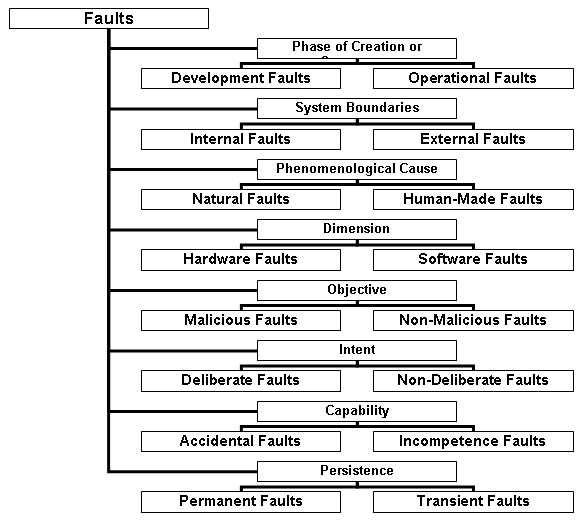
\includegraphics{icams1.png}}
        \caption{Elementary fault classes (redrawn from~\cite{b1})}
        \label{fig:1}
    \end{figure}

    Let us review some proposed definitions of survivability:

    \textbf{Definition 1:} Capability of a system to fulfill its mission, in a timely manner, in the presence of attacks, failures, or accidents~\cite{b3, b4, b5, b6}.

    \textbf{Definition 2:} The ability of a system to continue the adequate performance of its critical services and functions even after (unforeseen) successful attacks have taken place~\cite{b16}.

    \textbf{Definition 3:} The ability of an information system to continue to operate in the presence of faults, anomalous system behavior, or malicious attack~\cite{b14}.

    \textbf{Definition 4:} Robustness under conditions of intrusion, failure, or accident~\cite{b11}.

    \textbf{Definition 5:} Defined in terms of a survivable system where it ``must be adaptable, able to respond to attacks and achieve its goals''~\cite{b13}.

    According to~\cite{b1}, an attack is an operational, external, human-made, malicious and deliberate fault. It can be hardware/software, permanent/transient as well. An accident is a non-malicious, non-deliberate, and, of course, an accidental fault. It can be development/operational, internal/external, natural/human-made, hardware/software, permanent/transient as well. An intrusion is an external, human-made, malicious and deliberate fault. It can be development/operational, hardware/software, permanent/transient as well. The \textit{anomalous system behavior} mentioned in definition 3 is nothing but the error because error is defined as deviation in the expected behavior of the system that can result in failure.  Only when a fault, say intrusion or accident, causes a failure, the concept of survivability arises. Before the occurrence of failure, there is no difference between traditional dependability measures and the survivability. Therefore, most of design effort of a survivable system can be accomplished by the traditional techniques for designing dependable systems. Trends such a fault avoidance, fault tolerance and fault recovery can be used in the design of a survivable system. What remains, is the operation of the system after failure, which can be expressed using the survivability concept.

    The failure is usually defined as an event that occurs when the delivered service deviates from the correct or defined service. We should note that the failure is not a single state of the system, i.e. the failure can be time dependent. After occurrence of a failure, its severity can increase or decrease with respect to time. Therefore several states of failure should be considered based on their different severities. Once a failure occurred, the system is said to be failed, because it no longer delivers 100\% of its ideal service, but still its degree of service could be acceptable. The set of all failure states is called the \textit{failure-set}. In many applications, there are different states of failure that occur. There is a state that the system can not continue to work and it is \textit{halted}. Let's call this state of failure the \textit{Halt State}. The halt is the phase of a system that must be strictly avoided to let the system survive. In fact, the chance of exiting from the halt state (e.g. by repairing or recovery) is zero or so low that it can be neglected. Therefore, a new phase, which is Halt, can be added to the well-known chain of fault$\rightarrow$error$\rightarrow$failure as shown in Fig.~\ref{fig:2}. Now the concept of survivability can be analyzed in the framework of dependability and survivability is an attribute of dependability. The major role of survivability is between the failure and the halt but it is not restricted to this part. If a system tolerates faults, it postpones the halt, so the survivability increases. Fault recovery, fault masking, fault avoidance, error recovery and error masking can improve the overall survivability of the system. Some new techniques can be introduced such as failure recovery, failure masking or halt avoidance.

    \begin{figure}[htbp]
        \centering
        \makebox[\textwidth]{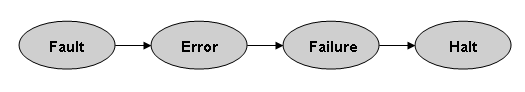
\includegraphics{icams2.png}}
        \caption{Cause-and-effect chain of dependability}
        \label{fig:2}
    \end{figure}

    The concept of survivability is related to two factors: i) the time between the occurrence of the failure and the time the system enters the halt state; ii) The degree of functionality of the system during this time with respect to the desired services in the specification of the system. In other words, more the deviation of delivered service from the correct service, less the system is survivable. One important question to answer is the relation between the reliability, availability or fault tolerance and the survivability.

    Consider an example: suppose that there are two airplanes, one has a very good reliability, i.e. it takes a long time for the first failure to occur, but once the failure occurred the airplane is supposed to crash and it cannot tolerate its failure. On the other hand, there is another airplane with a poor reliability and it encounters failures frequently. However, when the failure occurred there are some recovery mechanisms that can bring it to the normal working state before crashing (i.e. it oscillates between failed and healthy states).

    Now which one is more survivable? Obviously with this information we can't judge. Is the former more survivable because it is more reliable? Or is the latter more survivable because it has recovery mechanisms? We see that the concept of reliability is much related to that of survivability. This is true for other aspects of dependability such as fault tolerance and availability. By considering the Halt state, it can be seen that known dependability techniques such as fault avoidance, fault masking and fault tolerance improve the survivability as shown in Fig.~\ref{fig:3}. According to this figure, if a fault is avoided, the halt is avoided; if a fault is masked, the halt is avoided too, if a fault is tolerated; the halt is avoided as well; these all, indicate an improvement of the survivability. The main part of survivability concern arises after the failure.

    There are conditions that the failure can't be recovered immediately. However, in these conditions usually there is a force to recover the system as soon as possible and not let the failure to get worse. Therefore the answer to the question: ``how much and to what extent this system can tolerate a failure?'' is a measure of how survivable the system is. In the above mentioned airplanes example, the first airplane works well before failure, so it avoids halt. The second airplane works well between failure and halt, so it tolerates failure. Both systems are partly survivable; for them to be wholly survivable, a system must work well before failure, and between failure and halt, as well.

    \begin{figure}[htbp]
        \centering
        \makebox[\textwidth]{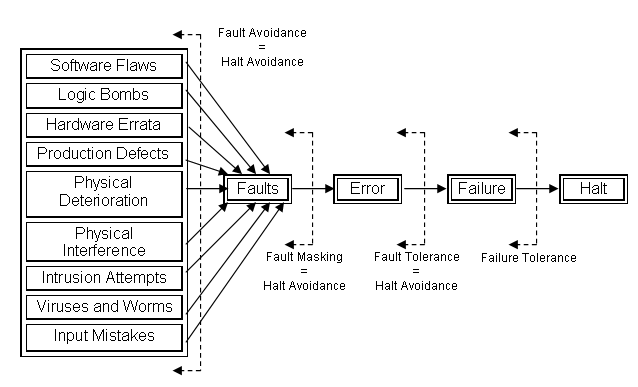
\includegraphics{icams3.png}}
        \caption{Relationship between fault-tolerance and survivability}
        \label{fig:3}
    \end{figure}

    \section{A Framework for Survivability Evaluation} \label{sec:fram}
    Let $r$ be the set of requirements that the system must satisfy or the set of goals that must be achieved. When the system starts to work, every element of $r$ i.e. the $r_i^{th}$ element is satisfied by some degree. Let $F$ be the set of some evaluating functions such that $F_i\left( t \right):\mathbb{R}^+\rightarrow\left[ 0,1 \right]$ where $\mathbb{R}^+$ is the set of all positive real numbers. $F_i\left( t \right)$ Specifies how much the $i^{th}$ requirement is satisfied at time $t$. Let $g\left( t \right):\mathbb{R}^+\rightarrow\left[ 0,1 \right]$ be a subsuming function that gives a measure of how totally the requirements of the system are satisfied at time $t$. ideally, the system is considered as working or non-failed when $g=1$. In fact, as long as all the requirements of the system are fully satisfied, the system is working properly and is not failed. Once the failure is occurred, $g$ will be less than $1$. $g$ may not be necessarily a fixed number; it could increase or decrease depending on how the recovery or repair operations are performed. If no recovery or repair operation is present, the system gets worse and consequently, $g$ decreases until it reaches zero.

    Using the above notations, we can define the following states:

    \textbf{Failure-Set:} Set of all states that $0\leq g \leq1$. This is a set consisting of all states in which all requirements are not satisfied completely.

    \textbf{Failure:} The first member of the failure-set in which the system enters. Note that, it is not necessarily equal to $\max\limits_{0 \leq g \leq 1}g$. Because, there may be two states of failure, with different $g$s, that the system may first enter only one of them (Fig.~\ref{fig:4}).

    \textbf{HT:} Halt Threshold, a value of g that any $g \leq HT$ is not acceptable.

    \textbf{Halt-Set:} Set of states in which  $0 \leq g \leq HT$ and we can't exit from it. In fact, the probability of exiting from this state is so low that can be considered as zero. Obviously they are states with a self-loop.

    \textbf{Halt:} The first member of the halt-set in which the system enters.

    Using the above definitions, we can define survivability as a function of two variables: $S\left( \bar{g},\bar{t} \right):\left[ 0,1 \right]\times \mathbb{R}^+ \rightarrow \left[ 0,1 \right]$ where $\bar{g}$ is the mean of $g$ and $\bar{t}$ is the mean time to reach the Halt state from the failure state.

    \begin{figure}[htbp]
        \centering
        \makebox[\textwidth]{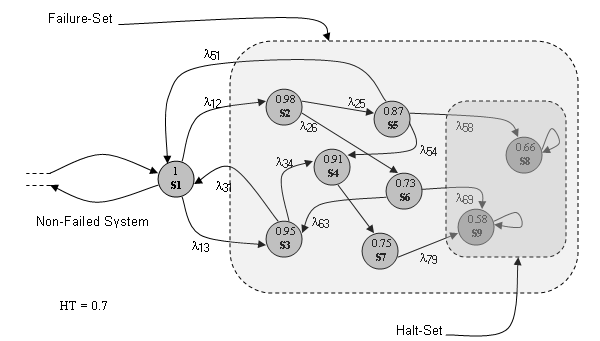
\includegraphics{icams4.png}}
        \caption{Different states after failure}
        \label{fig:4}
    \end{figure}

    \section{Conclusion} \label{sec:conc}
    A new framework has been proposed to evaluate the survivability of systems. Survivability can be integrated with dependability framework. Fault-error-failure chain is expanded to include the facet of survivability so that in addition to special survivability design techniques, all the design techniques used for dependable systems can be used in the design of survivable systems.

    \begin{thebibliography}{00}
        \bibitem{b1} A. Avizienis, J.C. Laprie, B. Randell, and C. Landwehr. Basic Concepts and Taxonomy of Dependable and Secure Computing. IEEE Transactions on Dependable and Secure Computing. 2004, 1(1).

        \bibitem{b3} I. Byon. Survivability of the U.S. Electric Power Industry. Master thesis, Carnegie Mellon University Pittsburgh, Pennsylvania, May 2000.

        \bibitem{b4} J. Caldera. Survivability Requirements for the U.S. Healthcare Industry. Master thesis, Carnegie Mellon University Pittsburgh, Pennsylvania, May 2000.

        \bibitem{b5} R.J. Ellison, D.A. Fisher, R.C. Linger, H.F. Lipson, T.A. Longstaff and N.R. Mead. An Approach to Survivable Systems. NATO IST Symposium on Protecting Information Systems in the 21st Century. 1999.

        \bibitem{b6} R.J. Ellison, R.C. Linger, H.F. Lipson, T.A. Longstaff and N.R. Mead. A Case study in Requirements for Survivable Systems. SEI. 2002.

        \bibitem{b7} H. Frank. Survivability analysis of command and control communications networks-part I\&II. IEEE Transactions on Communications. 1974, 22(5): 589-605.

        \bibitem{b8} M. Keshtgary. General Framework for networksurvivability performance evaluation. Ph.D. Dissertation, Sharif University of Technology, Dept. of Computer Eng, Tehran, Iran. 2005.

       \bibitem{b10} J.C. Knight, E. A. Strunk, K J. Sullivan . Towards a Rigorous Definition of Information System Survivability. Darpa Information survivability Conference and Exposition. Volume 1. 2003.

        \bibitem{b11} K. Kyamakya, K. Jobman, M. Meincke. Security and Survivability of Distributed Systems: An Overview. Proc. Of 21st Century Military Communications Conference, Volume 1, IEEE. 2000, pp. 1204-1208.

        \bibitem{b12} S.C. Liew and K.W. Lu. A framework for characterizing disaster-based network survivability. IEEE Journal on Selected Areas in Communications. 1994, 12(1): 52-58.

        \bibitem{b13} H. Shrobe. Model-Based Troubleshooting for Information Survivability. DARPA Information Survivability Conference and Exposition, Volume 2, IEEE. 1999, pp. 231-240.

        \bibitem{b14} J.M. Voas, A.K. Ghosh. Software Fault Injection for Survivability. DARPA Information Survivability Conference and Exposition. Volume 2, IEEE. 1999, pp. 256-270.

        \bibitem{b15} C. Wang, J. Davidson, J. Hill, J. Knight. Protection of Software-Based Survivability Mechanisms. the International Conference on Dependable Systems and Networks, IEEE. 2001, pp. 1413-1420.

        \bibitem{b16} M. Wilikens, T. Jackson. Survivability of Networked Information Systems and Infrastructures. European Commission Directorate.

        \bibitem{b18} A. Zolfaghari and F.J. Kaudel. Framework for network survivability performance. IEEE Journal on Selected Areas in Communications. 1994, 12(1): 46-51.

    \end{thebibliography}
\end{document}
